%!TEX root = ../thesis.tex
\section{Approaches to defect prediction}

We have already explored some approaches to code quality prediction. In this chapter we will highlight some methods, like \emph{BugCache}, \emph{FixCache} and \emph{Buggy Change Classification}, which are included in the type of approach we want to follow (\emph{change log}) and that allow us, together with other methods, to optimize defect localization.

\subsection{\emph{BugCache/FixCache}}

Based on the assumption that faults never occur isolated, and therefore where there's a defect others can also exist, \emph{BugCache} creates a list of components which have a high probability of containing defects, based on an analysis of the complete changes history of the project.

This algorithm stands out due to its precision, managing a 73 to 95\% accuracy when used with file-level granularity, being the best to date \cite{Kim2006}.

Defects are identified by order of occurrence and added to the list. When that list reaches its maximum size, components start to be removed according to the chosen substitution method. There are several methods using different metrics, such as \emph{Least Recent Used - LRU}, number of recent defects and number of recent changes \cite{Kim2006}.

With this algorithm, we can conclude \cite{Kim2006}:
%
\begin{itemize}
	\item If a defect has been introduced, there is a tendency to soon introduce additional new defects (\emph{temporal locality})
	\item If a component was added or changed recently, it has a higher probability of defect (\emph{changed-entity locality}, \emph{new-entity locality})
	\item If a component has introduced an error, the components most directly connected to that one will also introduce errors in the future (\emph{spatial locality})
\end{itemize}

The difference between \emph{BugCache} and \emph{FixCache} is the time at which each one updates the list. The former updates the list when a defect is introduced, while the latter only updates when the error is fixed. Due to this difference, implementing \emph{FixCache} is easier.

\subsection{\emph{Buggy Change Classification}}

\emph{Change Classification} has a notably different approach and a very distinct objective too. \emph{Change Classification}, resorting to \emph{Machine Learning} methods and available information about previous errors, is able to predict if a change has introduced a new defect. This prediction has a high accuracy of 78\% \cite{Whitehead2008}.

In a first phase, all changes up to that moment are either classified as \emph{buggy} or \emph{clean}. After classifying them and extracting data for each one, a model is created by \"training\" a classification algorithm.

The types of data used are divided in seven groups: complexity metrics, added code, removed code, file and folder names, new code and metadata \cite{Whitehead2008}.

Both \emph{Support Vector Machine} (SVM) and \emph{Naive Bayes} were used in the study, with the SVM-based classifier being the one with better results \cite{Whitehead2008}.

\subsection{Data-Augmented Software Diagnosis} \label{subsec:elmishali}

A different approach that also aims to help predict the location of software faults is Data-Augmented Software Diagnosis \cite{Elmishali}.

Model-based and spectrum-based approaches are able to identify faulty components with high precision and recall, but there is still room for improvement and since most projects use some kind of Version Control Software (VCS), there is a big amount of information that is not used. This opportunity is the foundation of the approach.

Barinel assumes that the defect probability, known as the prior, of every component is uniform, $0.001$. However, this approach proved it is possible to optimize Barinel results for Java projects by leveraging information about the project and supervised machine learning algorithms to predict the real component's defect probability.

First, healthy and faulty components are identified across the entire project's history according to Bug Trackers. For each component, a list of features, which is not specified, is extracted. The list is composed of traditional and object-oriented software complexity metrics, such as number of lines of code and cohesion, and values extracted from the software change history, like lines added or removed in last version and age of the file.

With the help of a supervised machine learning algorithm (either Random Forest, J48 or Naive Bayes) a model is created and used to classify each component in the project as healthy or buggy. The confidence that a component is faulty is then used as prior.

Experimental results revealed an increment both on precision and recall, see Figure \ref{fig:elmishali}. However, the solution was tested just on one project.
%
\begin{figure}%
    \centering
    \subfloat[Precision]{{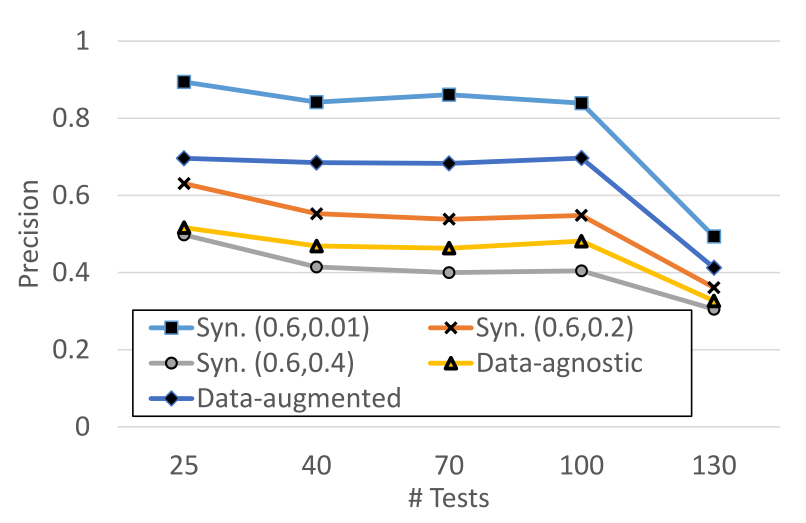
\includegraphics[width=0.4\textwidth]{elmishali-precision} }}%
    \qquad
    \subfloat[Recall]{{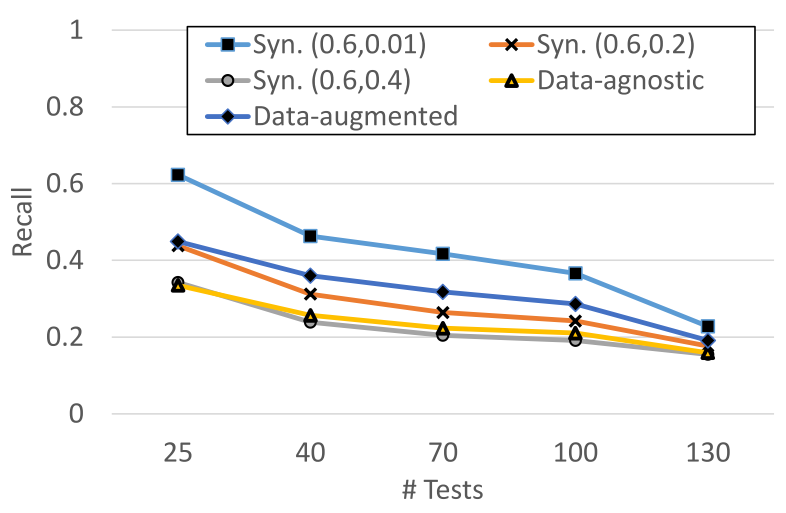
\includegraphics[width=0.4\textwidth]{elmishali-recall} }}%
    \caption{Diagnosis accuracy as a function of \# tests given to the diagnoser}%
    \label{fig:elmishali}%
\end{figure}
